\documentclass[tikz]{standalone}
\usetikzlibrary{calc}

\begin{document}
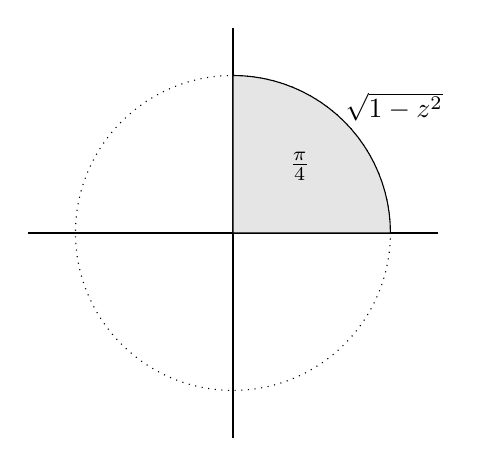
\begin{tikzpicture}[scale=2]
  \draw (-1.3, 0) -- (1.3, 0);
  \draw (0, -1.3) -- (0, 1.3);
  \draw[dotted] (0, 0) circle (1);
  \draw[fill=black!10, domain=0:90] plot
  ({cos(\x)}, {sin(\x)})
  -- (0, 0) -- cycle;
\node at (38:1.3) {$\sqrt{1-z^2}$};
\node at (45:0.6) {$\frac{\pi}{4}$};
\end{tikzpicture}
\end{document}
